\documentclass[11pt,a4paper,oneside,titlepage]{article}

\usepackage[english]{babel}
\usepackage{lineno,hyperref}
\usepackage[nolist]{acronym}
\usepackage[onehalfspacing]{setspace}
\usepackage{booktabs}
\usepackage{float}
\usepackage{amsmath}
\usepackage{listings}
\usepackage{color}
\usepackage{hyperref}
\usepackage{graphicx}
\usepackage{blindtext}
\usepackage{datetime}

\definecolor{LightGray}{gray}{0.70}
\lstdefinestyle{MctCpp}{%
    language=C++,
    keywordstyle=\bfseries,
    commentstyle=\itshape,
    rangeprefix=//--,rangesuffix=--,
    includerangemarker=false,
    columns=spaceflexible,
    escapeinside={/*@}{@*/},
    tabsize=4,
    frame=leftline,
    rulecolor=\color{LightGray},
    basicstyle=\ttfamily,
    numbers=left,
    numberstyle=\normalfont\tiny\color{LightGray},
    xleftmargin=0.75cm,
}

\lstdefinestyle{MctTxt}{%
    language={},
    keywordstyle=\bfseries,
    commentstyle=\itshape,
    rangeprefix=//--,rangesuffix=--,
    includerangemarker=false,
    columns=spaceflexible,
    escapeinside={/*@}{@*/},
    tabsize=4,
    frame=leftline,
    rulecolor=\color{LightGray},
    basicstyle=\ttfamily,
    numbers=left,
    numberstyle=\normalfont\tiny\color{LightGray},
    xleftmargin=0.75cm,
}

\textheight = 25cm
\textwidth = 15cm

\hoffset = -1cm
\voffset = -2cm


\begin{document}
%------------------------------------------------------------------------------
\newcommand{\CenFig}[2]{
    \begin{figure}[H]
        \begin{center}
            \includegraphics[width=#2\textwidth]{#1}
        \end{center}
    \end{figure}
}

\makeatletter
\lst@Key{matchrangestart}{f}{\lstKV@SetIf{#1}\lst@ifmatchrangestart}
\def\lst@SkipToFirst{%
    \lst@ifmatchrangestart\c@lstnumber=\numexpr-1+\lst@firstline\fi
    \ifnum \lst@lineno<\lst@firstline
        \def\lst@next{\lst@BeginDropInput\lst@Pmode
        \lst@Let{13}\lst@MSkipToFirst
        \lst@Let{10}\lst@MSkipToFirst}%
        \expandafter\lst@next
    \else
        \expandafter\lst@BOLGobble
    \fi}
\makeatother
%------------------------------------------------------------------------------
\newcommand{\FigCapLabSca}[4]{
\begin{figure}[H]
    \begin{center}
        \includegraphics[width=#4\textwidth]{#1}
        \caption[]{#2}
        \label{#3}
    \end{center}
\end{figure}
}
%
\thispagestyle{empty}
\begin{center}
    \begin{figure}[H]
        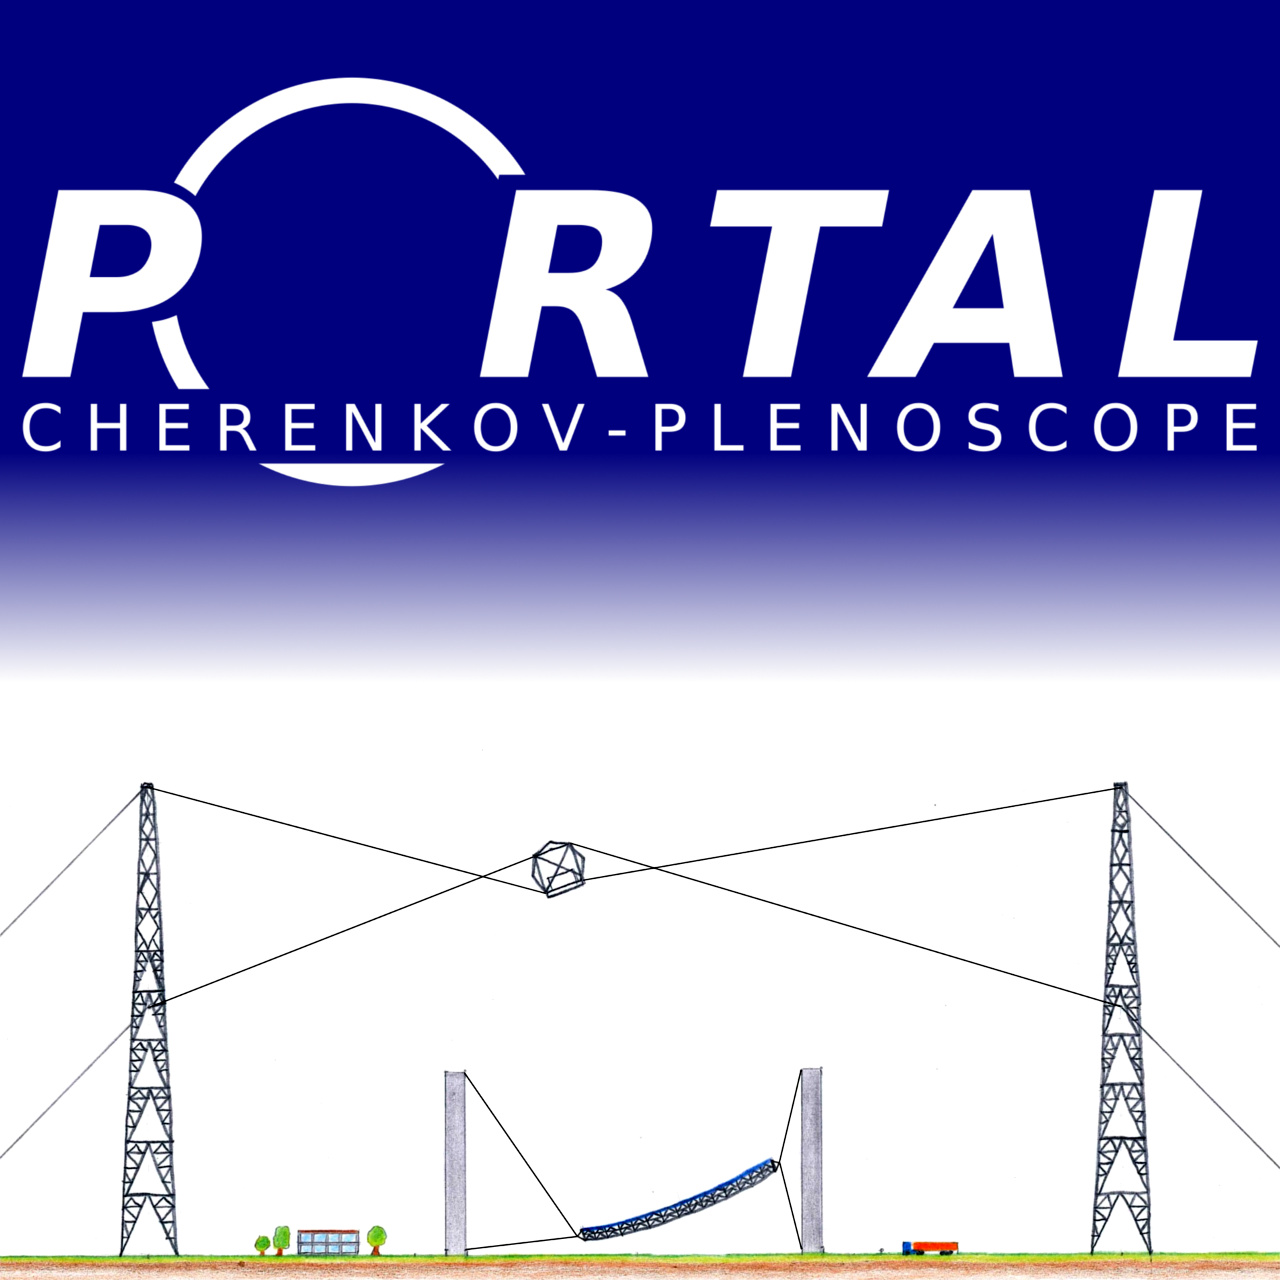
\includegraphics[width=1.0\textwidth]{figures/portal.jpg}
    \end{figure}
    \begin{huge}
        Technical Specifications
    \end{huge}
    \vfill
    \begin{Large}
        Sebastian Achim Mueller
    \end{Large}
    \\
    sebastian-achim.mueller@mpi-hd.mpg.de\\
    Division: Werner Hofmann\\
    \vspace{20pt}
    \par\smallskip\noindent
    Max-Planck-Institute for Nuclear Physics\\
    Saupfercheckweg 1\\
    69117 Heidelberg\\
    Germany\\
    \today
\end{center}
\newpage
%-------------------------------------------------------------
\pagenumbering{Roman}
\tableofcontents
%-------------------------------------------------------------
\cleardoublepage
%
\setcounter{page}{0}
\pagenumbering{arabic}
%
\linenumbers
\newcommand{\OutOfFocus}{\textit{out of focus}}
\newcommand{\InFocus}{\textit{in focus}}
\newcommand{\FocalRatio}{F}
\newcommand{\FocalLength}{f}
\newcommand{\ImageDistance}{b}
\newcommand{\ImageSensorDistance}{d}
\newcommand{\ObjectDistance}{g}
\newcommand{\ApertureDiameter}{D}
\newcommand{\ApertureFunction}{A}
\newcommand{\BokehFunction}{B}
\newcommand{\FieldOfView}{\alpha}
\newcommand{\BokehRadius}{r_\BokehFunction}
\newcommand{\BokehTemplateFunction}{\BokehFunction_{\text{template}}}
\newcommand{\ApertureRadius}{r_\ApertureFunction}
\newcommand{\zHy}{{z_\text{Hy}}}
\newcommand{\zPa}{{z_\text{Pa}}}
\newcommand{\zDC}{{z_\text{DC}}}
%-------------------------------------------------------------------------------
\section{Abstract}
%
The Plenoscope is a novel class of optical instrument which overcomes inherent limitations of the telescope.
%
Unlike the telescope, the plenoscope can accept misalignments and even deformations of its imaging-reflector as long as these are known.
%
Also the plenoscope turns the telescope's narrow depth-of-field into stereo observation-power.
%
Both these advantages might allow gamma-ray-astronomy to observe gamma-rays with energies at $1$ to $25\,$GeV from ground.
%
Today, this energy range is not well known to astronomy.
%
Sattelites only effectively detect gamma-rays up to energies of $1\,$GeV and Cherenkov-telescopes on ground only reach down to about $25\,$GeV.
%
The Cherenkov-Plenoscope might have the potential to close this gap.
%
Currently, we estimate the observation-power for gamma-rays of a specific Cherenkov-plenoscope named Portal with an aperture-diameter of $71\,$m.
%
\section{Possible Sites}
%
The Plenoscope shall be located at above 2,000\,m a.s.l. e.g. on the ALMA site in Chile or on Gamsberg in Namibia.
%
The site shall have dark night skies without arificial light polution.
%
We prefer the southern hemisphere.
%-------------------------------------------------------------------------------
\section{Target-Geometry}
%
All actuators, moving the dish and the sensor-plane, try to reach the target-geometry during operation.
%
We describe optics with respect to the imaging-reflector's frame.
%
The $z$-axis is the optical axis of the imaging-refelctor.
%
Table \ref{TabBasicDimensions} shows relative dimensions in arbitrary units.
%
The absolute dimensions range from aperture-diameters $\ApertureDiameter = 50\,$m to $100\,$m.
%
The size of the plenoscope is only limited by its cost and ultimatively the square-cube-law.
%
All optical properties only become better with larger sizes.
%
Fix design-keys of the plenoscope are its focal-ratio of $\FocalLength/\ApertureDiameter = 1.5$ and its field-of-view of $6.5^\circ\,$.
%
\begin{table}[H]
    \begin{center}
        \begin{tabular}{lr}
            \toprule
            aperture-diameter $\ApertureDiameter$ & $100\,$a.u.\\
            focal-length $\FocalLength$ & $150\,$a.u.\\
            F-number or foacal-ratio, $\FocalLength/\ApertureDiameter$ & $1.5$\\
            sensor-plane-distance $\ImageSensorDistance$ & $150$ to $\approx 160\,$a.u.\\
            sensor-plane's diameter & $17\,$a.u.\\
            sensor-plane-housing's diameter & $20.4\,$a.u.\\
            sensor-plane's field-of-view $\FieldOfView$ & $6.5^\circ\,$\\
            \bottomrule
        \end{tabular}
        \caption[]{Plenoscope's dimensions in arbitrary units (a.u.)}
        \label{TabBasicDimensions}
    \end{center}
\end{table}
%
The sensor-plane-distance
%
\begin{eqnarray}
\ImageSensorDistance &=& \frac{1}{\frac{1}{\FocalLength} - \frac{1}{\ObjectDistance}}
\end{eqnarray}
%
depends on the targeted object-distance which about $g \approx 10,000\,$m.
%
\subsection{Imaging-Reflector}
%
We use a segmented imaging-reflector with identical mirror-facets.
%
All mirror-facets have the same hexagonel aperture and focal-lenght $f$.
%
The $x$ and $y$ position of a mirror facet are defined by the hexagonal grid of the facets.
\CenFig{figures/2D_mirror_facets.png}{0.4}
%
The relative $z$-components of the mirror-facets are defined by a parabolic component
%
\begin{eqnarray}
    \zPa(r) &=& \frac{1}{4 \FocalLength} r^2,
\end{eqnarray}
%
which depends on the facet's distance $r$ to the optical-axis.
%
A global offset $q$ is added so that the position of the $i$-th facet is
%
\begin{eqnarray}
\label{eq_mirror_position}
\vec{m}_{i} &=& \begin{pmatrix}
                            r_i \cos(\varphi_{i})\\
                            r_i \sin(\varphi_{i})\\
                            \zPa_{i}(r_i) + q
                        \end{pmatrix}.
\end{eqnarray}
%
\FigCapLabSca{figures/mirror_facet_position_z.png}{$z$ positions of the facets}{FigFacetZ}{0.8}
%
The common offset $q$ is chosen so that the average distance between all the $N$ facet centers $\vec{m}$ and the focal-point $\vec{\FocalLength} = (0,0, \FocalLength)^T$ becomes the focal-lenght
%
\begin{eqnarray}
    \label{eq_correct_focus}
    \FocalLength &\stackrel{!}{=}& \frac{1}{N} \sum_{i}^N 
    %
    \left \vert 
    %
    \vec{m}_{i}- \vec{\FocalLength}\,
    %
    \right \vert.
    %
\end{eqnarray}
%
The $x$ and $y$ orientations are chosen so that the $i$-th mirror-facet's surface-normal
%
\begin{eqnarray}
\label{eq_facet_normal}
\vec{n}_{i} &=& \frac{2\vec{\FocalLength} - \vec{m_i}}{\vert 2\vec{\FocalLength} - \vec{m_i} \vert}
\end{eqnarray}
%
is pointing towards the $2$-$\vec{\FocalLength}$-point.
%
\CenFig{figures/mirror_facet_orientation.png}{0.8}
%
\subsection{Restricted Volumes}
%
To not block light, certain volumes should be kept free of obstacles.
%
Figure \ref{FigRestrictedArea} shows the restricted volumes on the plenoscope in yellow.
%
There is a blind cone in the center of the reflector which can be blocked to have additional support structures.
%
Support structres, that have to be in the restricted volumes, should be shaped so that the shadowing is minimal, e.g. using thin cables or flat structures which are elongated along the optical-axis.
%
\FigCapLabSca{figures/lebowsky_restricted_areas.png}{
    Objects in the yellow volume will block light. The more saturated the yellow, the more important it is to keep this volume free. Figure is to scale.
}{FigRestrictedArea}{0.68}
%
\subsection{Mirror-Facets}
%
All mirror-facets are interchangeable with each other.
%
The mirror-facets have all the same focal-lenght $\FocalLength$ and a hexagonal shape.
%
Table \ref{TabFacets} shows the properties of typical mirror-facets.
%
We will opt for the biggest facet which has proven to be mass producible, i.e. $2\,$m$^2$.
%
The weight of a two-axis-actuator for the facets is $\approx 5\,$kg/facet (almost) regardless of the size of the facet.
%
\begin{table}[H]
    \begin{center}
        \begin{tabular}{lccrrrrr}
            type designation & shape & $A$/m$^2$ & $s$/m & $m$/kg & $\rho_A$/kg\,m$^{-2}$ & $\rho_A$/kg\,m$^{-2}$\\
             & & & & & raw & with actuators\\
            \toprule
            MAGIC 1st gen. & square & 0.25 & 0.50  & 4.0 & 16.0 & 21.0\\
            MAGIC 2nd gen. & square & 0.96 & 1.00 & 13.4 & 14.0 & 19.2\\
            VERITAS        & hex    & 0.32 & 0.61 & 10.4 & 32.4 & 48.0\\
            FACT/HEGRA     & hex    & 0.32 & 0.61 & 5.5 & 17.6 & 33.7\\
            CTA MST INAF   & hex    & 1.25 & 1.20 & 25.0 & 20.0 & 24.0\\
            CTA LST INAF   & hex    & 1.97 & 1.50 & 45.0 & 22.8 & 25.3\\
            \bottomrule
        \end{tabular}
        \caption[]{Typical mirror-facets in Cherenkov-telescopes. $s$ is the spacing of the facets, i.e. the flat-to-flat-diameter of the hexagonal facets.}
        \label{TabFacets}
    \end{center}
\end{table}
%
\subsection{Sensor-Plane}
%
The sensor-plane has the shape of a disc.
%
We opt for \mbox{$\Delta \alpha \approx 0.067^\circ$} angular resolution.
%
The sensor-plane's diameter
%
\begin{eqnarray}
D_\text{sensor} &=& 2 \FocalLength \tan \left( \frac{\FieldOfView} {2}\right)
\end{eqnarray}
%
is defined by the targeted field-of-view $\FieldOfView$ and the focal-length $\FocalLength$.
%
We expect the sensor-plane's housing to have an overhead of $120\%$.
%
For $\ApertureDiameter=100\,$a.u. this yields to \mbox{$D_\text{sensor} = 17.04\,$a.u.} and a housing diameter of \mbox{$D_\text{sensor housing} = 20.45\,$a.u.}
%
We expect the electric compartment of the sensor-plane to be rather flat, maybe $2\,$a.u. to $4\,$a.u. in height.
%
Table \ref{TabFullImageSensors} shows typical dimensions of sensor-planes in Cherenkov-telescopes.
%
We expect the sensor-plane to be as lightweight as the lightest Cherenkov-Telescope sensor-planes, which is about $\rho_A = 600\,$kg/m$^2$.
%
\begin{table}[H]
    \begin{center}
        \begin{tabular}{lccrrrrr}
            type designation & $A$/m$^2$ & $m$/kg & $\rho_A$/kg\,m$^{-2}$\\
            \toprule
            CAT France & 0.19 & 110 & 560\\
            MAGIC      & 0.85 & 450 & 530\\
            VERITAS    & 0.42 & -- & -- \\
            FACT       & 0.12 & 175 & 1458\\
            HESS 1     & 1.35 & 800 & 593\\
            HESS 2     & 3.14 & 2800 & 891\\
            \bottomrule
        \end{tabular}
        \caption[]{Typical sensor-plane in Cherenkov-telescopes. Mass includes the housing.}
        \label{TabFullImageSensors}
    \end{center}
\end{table}
%-------------------------------------------------------------------------------
\section{Geometry-Margins}
%
The novel sensor-plane of the plenoscope can tollerate misalignments and displacements between the sensor-plane and the imaging-reflector.
%-----------
\subsection{Sensor-Plane relative to Imaging-Reflector}
%-----------
\subsubsection{$z$ Translation}
%
The translation in $z$ of the sensor-plane-distance with respect to its targeted position
%
\begin{eqnarray}
\Delta \ImageSensorDistance & = & \ImageSensorDistance_\text{actual} -\ImageSensorDistance_\text{target}
\end{eqnarray}
%
can be tolerated as long as it is known.
%
\CenFig{figures/image_sensor_displacement_z.png}{0.6}
%
\begin{table}[H]
    \begin{center}
        \begin{tabular}{lr}
            sensor-plane's translation $z$ & $\Delta \ImageSensorDistance$ /a.u.\\
            \toprule
            Mandatory & -4.6 $<$ $\Delta \ImageSensorDistance$ $<$ 7.9\\
            Good      & -2.3 $<$ $\Delta \ImageSensorDistance$ $<$ 3.8\\
            Perfect   & -1.1 $<$ $\Delta \ImageSensorDistance$ $<$ 1.9\\
            \bottomrule
        \end{tabular}
    \end{center}
\end{table}
%-----------
\subsubsection{$x$, $y$ Translation}
%
A translation $\Delta x$, $\Delta y$ can be tollerated, as long as the actual $x$ and $y$ positions are known.
%
\CenFig{figures/image_sensor_displacement_xy.png}{0.6}
%
\begin{table}[H]
    \begin{center}
        \begin{tabular}{lr}
            sensor-plane's translation in $x$, $y$ & $\Delta xy$ /a.u.\\
            \toprule
            Mandatory & $< 0.72$\\
            Good      & $< 0.36$\\
            Perfect   & $< 0.18$\\
            \bottomrule
        \end{tabular}
    \end{center}
\end{table}
%-----------
\subsubsection{Orientation $x$, $y$}
%
A misalignment $\beta$ of the optical-axis against the sensor-plane can be tollerated, when $\beta$ is known.
%
Our sensor-plane is able to reconstruct this misalignment, but it loses aperture-area $A_\text{eff}$.
%
\CenFig{figures/image_sensor_misalignment_xy_view_cone.png}{0.6}
%
\begin{table}[H]
    \begin{center}
        \begin{tabular}{lrr}
            sensor-plane misalignment $x$, $y$ & $\beta$/1$^\circ$ & $A_\text{eff}$/\%\\
            \toprule
            Mandatory & $< 3.0$ & 90.0\\
            Good      & $< 1.5$ & 95.0\\
            Perfect   & $< 0.75$ & 97.5\\
            \bottomrule
        \end{tabular}
    \end{center}
\end{table}
%-----------
\subsubsection{Orientation in $z$}
%
Any rotation in $z$ can be tolerated, as long as the rotations is known.
%-----------
\subsection{Deformation of Sensor-Plane}
%
The sensor-plane itself is assumed to be stiff, i.e. the sensor-plane plane does not bend or deform more than $0.05\,$a.u. across its diameter.
%-----------
\subsection{Deformation of Imaging-Reflector}
%
As a rule of thumb:
The miss orientation of a mirror facet against its target orientation, caused by deformations of the dish, shall not exceed \mbox{$\frac{\Delta \alpha}{2} \approx 0.034^\circ$}, i.e. half the sensor-plane's angular resolution.
%
\begin{eqnarray}
\arccos \left( \vec{n}_\text{target} \cdot \vec{n}_\text{actual} \right) &<& \frac{\Delta \alpha}{2}
\end{eqnarray}
%-----------
\subsubsection{Slow and Elastic Deformations}
%
When we use mirror-facets with individual actuators, we can accept slow, and elastic deformations of the dish even in excess of $\frac{\Delta \alpha}{2}$.
%
For example gravitational slump is often slow and elastic.
%
Slow means, that the mirror-facet's actuators can keep up with the deformations of the dish while the plenoscope is slowly tracking a source in the sky.
%
(The MAGIC actuators can tilt a mirror-facet with $0.5^\circ/$s).
%
Elastic means, that the deformation will be the same for a given pointing of the plenoscope.
%
The MAGIC Cherenkov-telescope successfully counteracts slow and elastic deformations.
%
In case there are no deformations $> \frac{\Delta \alpha}{2}$, we can drop the mirror-facet's individual actuators.
%-------------------------------------------------------------------------------
\section{Movements}
%<
The plenoscope has two different modes of operation.
%
A slow mode to observe sources on the sky dome, and a fast mode to switch between the sources.
%
We want to avoid singularities in the inverse kinematics, especially near the zenith.
%
For example, the zenith's singularity on the altitude-azimuth-mounts limits all Cherenkov-telescopes in the hunt for gamma-ray-bursts.
%-----------
\subsection{Fast Repositioning in any Geometry}
%
When the plenoscope is pointing to a different source on the sky dome, the sensor-plane is not recording and the target-geometry is not required.
%
A high speed repositioning of $90^\circ/$min would allow us to hunt gamma-ray-bursts.
%
\begin{table}[H]
    \begin{center}
        \begin{tabular}{lr}
            Fast repositioning velocity & $\dot{\Theta}$/$1^\circ$\,min$^{-1}$\\
            \toprule
            Mandatory & 23\\
            Good      & 45\\
            Perfect   & 90\\
            \bottomrule
        \end{tabular}
    \end{center}
\end{table}
%-------------------------------------------------------------------------------
\subsection{Slow Tracking in Target-Geometry}
%
When the plenoscope is slowly tracking a source on the sky dome, it is only counteracting the rotation of the earth \mbox{$\dot{\Theta}_\text{Earth} = 0.25^\circ/$min}.
%
During slow tracking, the plenoscope has be in its target-geometry.
%
The plenoscope sensor-plane is only recording during this slow tracking mode.
%
For some observations, it is useful to move around a source in a spiral movement, which demands for tracking-velocities $\dot{\Theta}$ three times higher than $\dot{\Theta}_\text{Earth}$.
%
\begin{table}[H]
    \begin{center}
        \begin{tabular}{lr}
            Tracking velocity in target-geometry & $\dot{\Theta}/1^\circ$\,min$^{-1}$\\
            \toprule
            Mandatory & 0.25\\
            Good      & 0.5\\
            Perfect   & 0.75\\
            \bottomrule
        \end{tabular}
    \end{center}
\end{table}
%-----------
\subsection{Maximum Zenith-Distance}
%
The plenoscope should reach a zenith-distances $\Theta$ of $45\,^\circ$ in order to cover a large solid angle in the sky.
%
\begin{table}[H]
    \begin{center}
        \begin{tabular}{lr}
            Zenith-distance & $\Theta$/1$^\circ$\\
            \toprule
            Mandatory & 30\\
            Good      & 45\\
            Perfect   & 60\\
            \bottomrule
        \end{tabular}
    \end{center}
\end{table}
%-------------------------------------------------------------------------------
\section{Tracking of the Actual Geometry}
%
All translations and misalignments of the sensor-plane with respect to the imaging-reflector can only be tollerated when they are tracked and known.
%
We need a sampling-rate one order-of-magnitude higher than the dominant Eigenfrequencies of the structure.
%
The MAGIC-telescope's arch has an Eigenfrequency of $\approx 1\,$Hz.
%
Assuming that the dominant Eigenfrequencies on a big plenoscope will not be higher, a sampling rate $f_\text{sample}$ of $10\,$Hz might be sufficient.
%
\begin{table}[H]
    \begin{center}
        \begin{tabular}{lr}
            Sampling rate & $f_\text{sample}$/Hz\\
            \toprule
            Mandatory & 10\\
            Good      & 25\\
            Perfect   & 50\\
            \bottomrule
        \end{tabular}
    \end{center}
\end{table}
%
\begin{table}[H]
    \begin{center}
        \begin{tabular}{lr}
            sensor-plane $x$, $y$ and $z$ tracking accuracy &/a.u.\\
            \toprule
            Mandatory & $\pm$ $7.2 \cdot 10^{-2}$\\
            Good      & $\pm$ $3.6 \cdot 10^{-2}$\\
            Perfect   & $\pm$ $1.8 \cdot 10^{-2}$\\
            \bottomrule
        \end{tabular}
    \end{center}
\end{table}
%
\begin{table}[H]
    \begin{center}
        \begin{tabular}{lr}
            sensor-plane tilt in $x$, $y$ ($\beta$), and $z$ tracking accuracy & /1$^\circ$\\
            \toprule
            Mandatory & $\pm$ 0.03\\
            Good      & $\pm$ 0.02\\
            Perfect   & $\pm$ 0.015\\
            \bottomrule
        \end{tabular}
    \end{center}
\end{table}
%
The tracking's implementation shall be able to work in the dark night without artificial illumination.
%
When artificial light is mandatory, it must not occupie the wavelength range from $200\,$nm to $\approx 800\,$nm.
%
The duty cycle of the illumination shall be below $1\cdot10^{-3}$.
%-------------------------------------------------------------------------------
\section{Maintanace}
%
The surfaces of the mirror-facets degrade over time, and the actuators of the facets will break over time.
%
Therefore the mirror-facets and their individual actuators shall be reachable from below for maintenance.
%-------------------------------------------------------------------------------
\section{Threat due to Sunlight}
%
The imaging-reflector of the plenoscope can be a threat when it projects the image of the sun onto near by objects.
%
For a focal-ratio of 1.5, the imaging-reflector can project an image of the sun with up to $6\,$MW/m$^2$.
%
\begin{eqnarray}
\frac{I_\text{sun image}}{I_\text{solar constant}} = \frac{_\text{aperture area}}{_\text{image area}} = \frac{(D^2/4) \pi}{(D F \tan(0.25^\circ))^2 \pi} 
\end{eqnarray}
%
When we go for a mount where the sensor-plane is mounted independent of the imaging-reflector, we can profit from separating the sensor-plane from the imaging-reflector to park it in a save position.
%
As long as the imaging-reflector lies flat on the ground, it can not incinerate objects on the ground.
%
However, it might still heat up the nearby support-structures.
%
We favor solutions which do not need additional mechanics, like e.g. domes or lids.
%-------------------------------------------------------------------------------
\section*{Acknowledgement}
%
This work profited from discussions with:
%
Adrian Biland, Werner Hofmann, Max Ludwig Ahnen, Dominik Neise, Spyridon Daglas, Eleni Chatzi, Axel Arbet Engels, and Felicitas Pauss.
%
The Cherenkov-plenoscope would not be possible without the current support by: Werner Hofmann and the Max Planck Institute for Nuclear Physics, and the crucial early support by Adrian Biland and the ETH-Zurich's Institute for Particle Physics and Astronomy.
%
%--references--
%\renewcommand{\bibname}{References}
%\bibliography{mct}
%\bibliographystyle{plain}
%\addcontentsline{toc}{chapter}{\bibname}
%
%--Appendix--
\end{document}